\documentclass[10pt]{beamer}

% Tema Limpo e Profissional
\usetheme{Madrid}
\usecolortheme{whale}

% Pacotes Essenciais
\usepackage[utf8]{inputenc}
\usepackage[portuguese]{babel}
\usepackage{graphicx}
\usepackage{booktabs}
\usepackage{amsmath}
\usepackage{amssymb}
\usepackage{listings}
\usepackage{xcolor}

% Configuracoes de Codigo (Python)
\lstset{
    language=Python,
    basicstyle=\ttfamily\scriptsize,
    keywordstyle=\color{blue}\bfseries,
    stringstyle=\color{orange},
    commentstyle=\color{gray!80!black}\itshape,
    breaklines=true,
    showstringspaces=false,
    backgroundcolor=\color{gray!5},
    frame=single,
    rulecolor=\color{gray!30},
    numbers=left,
    numberstyle=\tiny\color{gray},
    stepnumber=1,
    numbersep=5pt
}

% Metadados da Apresentacao
\title[Python - Funções]{Introdução às Funções em Python}
\subtitle{Automatizando Tarefas como Administradores de Redes}
\author[Prof. Reginaldo]{Prof. Reginaldo Fernandes\texorpdfstring{\\ \small{Programação de Computadores}}{}}
\institute[IFCE]{Instituto Federal do Ceará -- Campus Tauá \\ Curso Técnico em Redes de Computadores}
\date{\today}

\begin{document}

% Slide de Titulo
\begin{frame}
    \titlepage
\end{frame}

% Sumario
\begin{frame}{Sumário da Aula}
    \tableofcontents
\end{frame}

% Blocos Modulares de Slides
\section{Introdução às Funções}

\begin{frame}{O Problema: Repetição Ineficiente}
    Imagine que você é o administrador de rede do IFCE Campus Tauá. Você precisa exibir uma mensagem de alerta no terminal do servidor toda vez que:
    \begin{itemize}
        \item Um usuário fizer login no sistema.
        \item Uma conexão cair.
        \item Um backup for concluído.
    \end{itemize}
    \vspace{0.3cm}
    Sem funções, você teria que copiar e colar o mesmo código várias vezes:
    \begin{block}{Código Repetitivo (Sem Funções)}
        \texttt{print("==============================")}\\
        \texttt{print(" ALERTA DE SEGURANCA DA REDE ")}\\
        \texttt{print("==============================")}
    \end{block}
    \textbf{Problema:} Se você quiser mudar o texto para "ALERTA DE SISTEMA", terá que alterar em todas as partes do código!
\end{frame}

\begin{frame}{O que é uma Função?}
    Na programação, uma \textbf{função} é um bloco de código que executa uma tarefa específica e pode ser reutilizado a qualquer momento.
    
    \begin{columns}
        \begin{column}{0.5\textwidth}
            \textbf{Analogias de Redes:}
            \begin{itemize}
                \item \textbf{Um Comando do Switch:} Quando você digita \texttt{ping}, há um código interno complexo rodando, mas você só vê o nome \texttt{ping}.
                \item \textbf{Servidor DHCP:} Recebe o endereço físico (MAC) e \textbf{retorna} um IP configurado.
            \end{itemize}
        \end{column}
        \begin{column}{0.5\textwidth}
            \begin{center}
                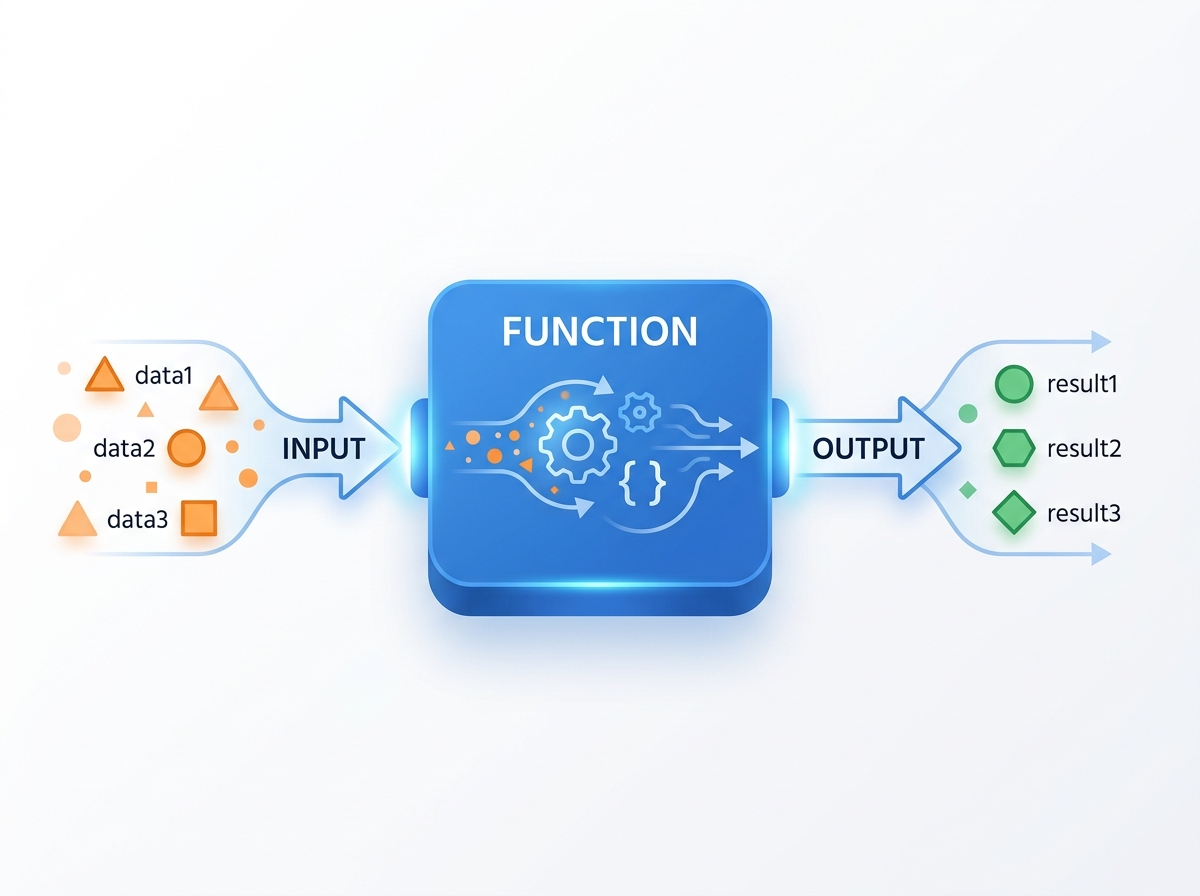
\includegraphics[width=0.8\textwidth]{diagrama_funcao.jpg} \\
                \footnotesize{Entrada (IP/Dados) $\rightarrow$ Processamento $\rightarrow$ Saída (Resultado)}
            \end{center}
        \end{column}
    \end{columns}
\end{frame}

\begin{frame}[fragile]{Como Definir uma Função em Python}
    Para criar uma função, usamos a palavra-chave \textbf{def} (de \textit{define} ou definir), seguida pelo nome da função, parênteses e dois pontos.
    
    \begin{lstlisting}[language=Python]
def nome_da_funcao(parametro1, parametro2):
    # Corpo da funcao (o que ela faz)
    # Codigo identado
    return resultado # Opcional
    \end{lstlisting}
    
    \vspace{0.3cm}
    \textbf{Regras importantes:}
    \begin{itemize}
        \item O nome deve ser explicativo (ex: \texttt{verificar\_conexao}).
        \item O bloco de código interno \textbf{deve estar identado} (com 4 espaços).
        \item Para executar a função, nós a ``chamamos'' pelo nome: \texttt{nome\_da\_funcao()}.
    \end{itemize}
\end{frame}

\section{Funções Sem Parâmetros e Sem Retorno}

\begin{frame}[fragile]{1. Sem Parâmetros e Sem Retorno}
    Essas funções executam tarefas fixas. Elas não precisam de nenhuma informação externa para rodar (sem parâmetros) e não devolvem valores para o programa principal (sem retorno).
    
    \vspace{0.3cm}
    \textbf{Analogia de Redes:}
    \begin{itemize}
        \item É como o comando \texttt{clear} no terminal do Linux ou \texttt{show clock} no switch Cisco.
        \item Você digita o comando, ele executa uma ação na tela, mas não te dá nenhum dado para guardar em uma variável.
    \end{itemize}
    
    \vspace{0.3cm}
    \textbf{Sintaxe:}
    \begin{lstlisting}[language=Python]
def minha_funcao():
    # Executa acao direta
    print("Acao executada!")
    \end{lstlisting}
\end{frame}

\begin{frame}[fragile]{Exemplo 1: Banner da Rede do IFCE}
    Vamos criar uma função para exibir o cabeçalho de boas-vindas do terminal da rede do campus.
    
    \begin{lstlisting}[language=Python]
def exibir_banner():
    # Exibe cabecalho estatico no console da rede
    print("+" + "-"*40 + "+")
    print("|   SISTEMA DE GERENCIAMENTO DE REDES    |")
    print("|         IFCE CAMPUS TAUA               |")
    print("+" + "-"*40 + "+")

# Como utilizar a funcao no script principal:
exibir_banner()
    \end{lstlisting}
    
    \vspace{0.2cm}
    \textbf{Resultado no Terminal:}
    \begin{block}{Saída}
        \texttt{+----------------------------------------+}\\
        \texttt{|   SISTEMA DE GERENCIAMENTO DE REDES    |}\\
        \texttt{|         IFCE CAMPUS TAUA               |}\\
        \texttt{+----------------------------------------+}
    \end{block}
\end{frame}

\begin{frame}[fragile]{Exemplo 2: Alerta de Reinicialização}
    Função para exibir um aviso sonoro (usando caracteres de alerta) e aviso de texto que o roteador principal será reiniciado.
    
    \begin{lstlisting}[language=Python]
def avisar_reboot():
    # Emite aviso sobre desligamento do roteador
    print("[ATENCAO] O Roteador Central sera reiniciado em 5 minutos!")
    print("Por favor, salvem as configuracoes pendentes.")
    print("Todas as conexoes ativas serao interrompidas.")

# Simulando o agendamento de manutencao:
print("Iniciando rotina de manutencao...")
avisar_reboot()
    \end{lstlisting}
    
    \vspace{0.2cm}
    \textbf{Saída:}
    \begin{block}{Saída}
        \texttt{Iniciando rotina de manutencao...}\\
        \texttt{[ATENCAO] O Roteador Central sera reiniciado em 5 minutos!}\\
        \texttt{Por favor, salvem as configuracoes pendentes.}\\
        \texttt{Todas as conexoes ativas serao interrompidas.}
    \end{block}
\end{frame}

\section{Funções Com Parâmetros e Sem Retorno}

\begin{frame}[fragile]{2. Com Parâmetros e Sem Retorno}
    Essas funções aceitam dados de entrada (chamados de \textbf{parâmetros} ou \textbf{argumentos}) para personalizar sua execução. Contudo, elas apenas realizam a ação e não devolvem um valor final ao programa.
    
    \vspace{0.3cm}
    \textbf{Analogia de Redes:}
    \begin{itemize}
        \item Pense no comando \texttt{ping 8.8.8.8}. O IP \texttt{8.8.8.8} é o parâmetro. Se você mudar o parâmetro para \texttt{192.168.1.1}, a função faz a mesma tarefa básica (enviar pacotes), mas direcionada a outro destino.
        \item O comando exibe as linhas na tela, mas você não armazena a resposta em uma variável do Python.
    \end{itemize}
    
    \vspace{0.3cm}
    \textbf{Sintaxe:}
    \begin{lstlisting}[language=Python]
def minha_funcao(parametro):
    # Usa o parametro para realizar uma acao
    print(f"Processando dado: {parametro}")
    \end{lstlisting}
\end{frame}

\begin{frame}[fragile]{Exemplo 1: Simulador de Ping}
    Vamos criar uma função que simula o utilitário \texttt{ping} (que usa pacotes ICMP -- \textit{Internet Control Message Protocol}) para testar a conectividade de um IP.
    
    \begin{lstlisting}[language=Python]
def ping(ip_destino):
    # Simula o teste de conectividade ICMP
    print(f"Disparando contra {ip_destino} com 32 bytes de dados:")
    print(f"Resposta de {ip_destino}: bytes=32 tempo=12ms TTL=64")
    print(f"Resposta de {ip_destino}: bytes=32 tempo=10ms TTL=64")
    print(f"Estatisticas do Ping para {ip_destino}: Concluido com sucesso.")

# Utilizando a funcao com alvos diferentes:
ping("10.0.0.1")
print("-" * 30)
ping("google.com")
    \end{lstlisting}
\end{frame}

\begin{frame}[fragile]{Exemplo 2: Bloqueio de Portas no Firewall}
    Função para simular o bloqueio de portas vulneráveis no Firewall do switch, registrando o motivo de segurança.
    
    \begin{lstlisting}[language=Python]
def bloquear_porta(porta, motivo):
    # Simula comando para bloquear porta no Firewall
    print(f"[FIREWALL] BLOQUEADO: Trafego na porta TCP {porta} suspenso.")
    print(f"[MOTIVO] Alerta de seguranca: {motivo}")
    print("Regra aplicada com sucesso na tabela IPTables.")

# Bloqueando portas suspeitas na rede da escola
bloquear_porta(21, "Tentativas excessivas de login no FTP")
print("-" * 30)
bloquear_porta(23, "Protocolo Telnet nao criptografado detectado")
    \end{lstlisting}
\end{frame}

\section{Funções Sem Parâmetros e Com Retorno}

\begin{frame}[fragile]{3. Sem Parâmetros e Com Retorno}
    Essas funções não necessitam de informações externas para iniciar. No entanto, ao finalizarem seu processamento, elas \textbf{devolvem (retornam)} um resultado para o programa principal usando a palavra-chave \textbf{return}.
    
    \vspace{0.3cm}
    \textbf{Analogia de Redes:}
    \begin{itemize}
        \item É como a placa de rede de um computador buscando seu próprio endereço físico (Endereço MAC -- \textit{Media Access Control}). O script da placa não precisa de entrada para descobrir seu próprio MAC, mas ela precisa devolver esse valor para o sistema operacional poder usá-lo nas comunicações.
        \item O valor retornado é guardado em uma variável para uso futuro.
    \end{itemize}
    
    \vspace{0.3cm}
    \textbf{Sintaxe:}
    \begin{lstlisting}[language=Python]
def obter_dado():
    resultado = "Informacao Interna"
    return resultado
    \end{lstlisting}
\end{frame}

\begin{frame}[fragile]{Exemplo 1: Endereço de Loopback}
    Vamos criar uma função que retorna o IP de loopback padrão da máquina local (\texttt{127.0.0.1}), usado para testes locais de rede.
    
    \begin{lstlisting}[language=Python]
def obter_ip_loopback():
    # Retorna o IP padrao para testes locais
    ip_local = "127.0.0.1"
    return ip_local

# Capturando o valor de retorno em uma variavel:
meu_teste = obter_ip_loopback()

print(f"Iniciando conexao de teste no host: {meu_teste}")
# Agora podemos usar a variavel para disparar conexoes
    \end{lstlisting}
    
    \vspace{0.2cm}
    \textbf{Nota didática:} A função \texttt{obter\_ip\_loopback()} não recebeu nada entre os parênteses, mas entregou um texto contendo o IP ao ser executada.
\end{frame}

\begin{frame}[fragile]{Exemplo 2: Gerador de Chave SSH Provisória}
    Esta função gera uma senha de acesso rápido de administrador para o SSH (geração de string com números aleatórios) para fins de teste temporário.
    
    \begin{lstlisting}[language=Python]
import random

def gerar_token_ssh():
    # Gera uma chave numerica aleatoria para sessao SSH
    token = random.randint(100000, 999999)
    return token

# Solicita uma nova chave para o analista de redes:
chave_acesso = gerar_token_ssh()

print("--- SOLICITACAO DE CREDENCIAIS ---")
print(f"Sua chave SSH provisoria eh: {chave_acesso}")
print("Esta chave expira em 60 segundos.")
    \end{lstlisting}
\end{frame}

\section{Funções Com Parâmetros e Com Retorno}

\begin{frame}[fragile]{4. Com Parâmetros e Com Retorno}
    Este é o tipo mais completo e comum de função. Ela \textbf{recebe} dados de entrada para trabalhar, executa o processamento matemático ou lógico e \textbf{retorna} o resultado final para o programa.
    
    \vspace{0.3cm}
    \textbf{Analogia de Redes:}
    \begin{itemize}
        \item Pense em uma \textbf{Calculadora de Sub-Rede}: Você insere o endereço IP e a máscara CIDR (\textit{Classless Inter-Domain Routing}) (parâmetros), a função realiza os cálculos binários (processamento) e te entrega a quantidade de hosts válidos na rede (retorno).
        \item É como um roteador decidindo rotas: entra o IP de destino $\rightarrow$ processa na tabela $\rightarrow$ retorna a interface de saída.
    \end{itemize}
    
    \vspace{0.3cm}
    \textbf{Sintaxe:}
    \begin{lstlisting}[language=Python]
def calcular_soma(a, b):
    resultado = a + b
    return resultado
    \end{lstlisting}
\end{frame}

\begin{frame}[fragile]{Exemplo 1: Conversor de Mbps para Kbps}
    Para configurar a largura de banda (\textit{bandwidth}) de interfaces em roteadores Cisco, muitas vezes precisamos informar o valor em Kilobits por segundo (Kbps). Vamos criar uma função que converte Megabits por segundo (Mbps) para Kbps.
    
    \begin{lstlisting}[language=Python]
def converter_mbps_para_kbps(mbps):
    # Converte largura de banda para configuracao de interfaces
    kbps = mbps * 1024
    return kbps

# Configurando um link de internet de 50 Mbps:
banda_config = converter_mbps_para_kbps(50)

print(f"Comando Cisco: bandwidth {banda_config}")
# Saida: Comando Cisco: bandwidth 51200
    \end{lstlisting}
\end{frame}

\begin{frame}[fragile]{Exemplo 2: Classificador de IPs (Público vs Privado)}
    Função que recebe um IP como string e verifica se ele pertence às faixas privadas comuns de redes locais (\texttt{192.168.x.x} ou \texttt{10.x.x.x}), retornando \texttt{True} se for privado e \texttt{False} se for público.
    
    \begin{lstlisting}[language=Python]
def verificar_ip_privado(ip):
    # Verifica se o IP fornecido eh da rede privada local
    if ip.startswith("192.168.") or ip.startswith("10."):
        return True
    else:
        return False

# Testando pacotes vindos da Internet e da Intranet:
ip_origem1 = "192.168.1.50"
ip_origem2 = "8.8.8.8"

print(f"O IP {ip_origem1} eh privado? {verificar_ip_privado(ip_origem1)}")
print(f"O IP {ip_origem2} eh privado? {verificar_ip_privado(ip_origem2)}")
    \end{lstlisting}
\end{frame}

\section{Resumo e Atividade Prática}

\begin{frame}{Tabela Resumo dos Tipos de Funções}
    Aqui está o mapa mental para você nunca mais esquecer os tipos de funções no Python:
    
    \vspace{0.4cm}
    \begin{table}
        \centering
        \begin{tabular}{lccl}
            \toprule
            \textbf{Tipo de Função} & \textbf{Entrada?} & \textbf{Saída?} & \textbf{Exemplo Prático (Redes)} \\
            \midrule
            Sem Param. e Sem Ret. & Não & Não & \texttt{exibir\_banner()} \\
            Com Param. e Sem Ret. & Sim & Não & \texttt{ping("10.0.0.1")} \\
            Sem Param. e Com Ret. & Não & Sim & \texttt{obter\_ip\_loopback()} \\
            Com Param. e Com Ret. & Sim & Sim & \texttt{verificar\_ip\_privado(ip)} \\
            \bottomrule
        \end{tabular}
        \caption{Comparação dos quatro tipos de funções em Python.}
    \end{table}
\end{frame}

\begin{frame}{Por que usar Funções? (Boas Práticas)}
    Como técnicos em redes, sabemos que a organização evita desastres (como cabos espalhados no rack!). No código, é a mesma coisa:
    
    \vspace{0.3cm}
    \begin{itemize}
        \item \textbf{Evita Duplicação (Princípio DRY - Don't Repeat Yourself):} Escreva uma vez, use quantas vezes quiser.
        \item \textbf{Facilidade de Manutenção:} Se o cálculo da sub-rede mudar, você altera apenas dentro da função, e não em centenas de linhas de código.
        \item \textbf{Organização e Legibilidade:} O código fica estruturado em módulos fáceis de ler, parecendo comandos do sistema operacional.
    \end{itemize}
\end{frame}

\begin{frame}[fragile]{Laboratório de Redes: Mini Desafio}
    \textbf{Exercício de Fixação:} Crie um script Python que automatize a verificação de uma lista de IPs da rede escolar.
    
    \begin{lstlisting}[language=Python]
# 1. Crie uma funcao que recebe um IP e retorna se ele esta ativo
# (Para o teste, retorne True se o IP terminar com par e False se impar)
def testar_host(ip):
    ultimo_octeto = int(ip.split(".")[-1])
    if ultimo_octeto % 2 == 0:
        return True
    return False

# 2. Varra uma lista de IPs e use a funcao criada para exibir o status
ips_rede = ["192.168.1.10", "192.168.1.15", "192.168.1.20"]

for ip in ips_rede:
    if testar_host(ip):
        print(f"Host {ip} -> ONLINE")
    else:
        print(f"Host {ip} -> OFFLINE")
    \end{lstlisting}
\end{frame}

\begin{frame}{Conclusão: Próximos Passos}
    \begin{center}
        \LARGE \textbf{Parabéns! Você deu o primeiro passo na Automação de Redes!} \\
        \vspace{0.5cm}
        \normalsize Na próxima aula de Programação de Computadores, vamos integrar essas funções com a biblioteca \texttt{socket} para interagir com roteadores de verdade na nossa rede local! \\
        \vspace{0.8cm}
        \textbf{Dúvidas?} \\
        \texttt{reginaldo.fernandes@ifce.edu.br}
    \end{center}
\end{frame}


\end{document}
